\section{LE3 -- Netzwerk-Modellierung \& Filterung}

\subsection{Ziel}
Dieses Kapitel dokumentiert die Konstruktion verschiedener Netzwerktypen aus den Fussballdaten sowie die angewandten Filterungstechniken zur Netzwerkreduktion. Basierend auf den Erkenntnissen aus dem EDA erstellen wir vier Netzwerke: Pass-Netzwerke (Spieler--Spieler), Match-Netzwerke (Team--Team), bipartite Spieler--Team-Netzwerke sowie ein Feld-Lokationsnetzwerk (Zone--Zone). Zusätzlich demonstrieren wir die Projektion von Two-Mode-Netzwerken auf One-Mode-Netzwerke und diskutieren die Auswirkungen auf Dichte und Skalierbarkeit.

\subsection{Netzwerkdefinitionen}

\subsubsection{Pass-Netzwerke (Spieler-zu-Spieler)}

\textbf{Netzwerktyp:} Gerichtet, Gewichtet

\textbf{Knoten:} Spieler (eindeutige \texttt{wyId}).

\textbf{Kanten:} Gerichtete Kanten von Passgebern zu Passempfängern. Eine Kante $(u, v)$ existiert, wenn Spieler $u$ erfolgreich einen Pass zu Spieler $v$ gespielt hat.

\textbf{Wesentliche Attribute:} Kanten werden primär über \texttt{pass\_count} (Gewicht) beschrieben. Ergänzend speichern wir (wo sinnvoll) aggregierte Kantenstatistiken wie Distanz und Winkel.

\textbf{Konstruktionsmethode:}
Die Identifikation des Passempfängers erfolgt über ein Matching auf der Eventsequenz. Für jeden erfolgreichen Pass wird der Empfänger als der Spieler identifiziert, der
\begin{itemize}
  \item im selben Team spielt,
  \item nicht der Passgeber ist,
  \item die nächste Aktion innerhalb eines Distanzschwellenwerts von 5 Metern zum Passendpunkt ausführt,
  \item und diese Aktion innerhalb eines Zeitschwellenwerts von 5 Sekunden nach dem Pass ausführt.
\end{itemize}

Die Heuristik ist relativ Robust, sie kann aber bei sehr schnellen Sequenzen oder quasi simultanen Aktionen Fehlzuordnungen verursachen und nicht immer garantieren, einen Empfänger ausfindig zu machen.

\subsubsection{Match-Netzwerke (Team-zu-Team)}

\textbf{Netzwerktyp:} Gerichtet, Gewichtet

\textbf{Knoten:} Fussballteams

\textbf{Kanten:} Gerichtete Kanten zwischen Teams basierend auf Spielergebnissen. Eine Kante $(A, B)$ repräsentiert Spiele, in denen Team $A$ gegen Team $B$ angetreten ist.

\textbf{Kantenattribute:}
\begin{itemize}
  \item \texttt{weight}: Gesamtanzahl der Tore von Team $A$ gegen Team $B$
  \item \texttt{matches}: Anzahl gespielter Spiele
  \item \texttt{wins}, \texttt{losses}, \texttt{draws}: Anzahl Siege, Niederlagen, Unentschieden
  \item \texttt{weight\_normalized}: Durchschnittliche Tore pro Spiel
\end{itemize}

\textbf{Knotenattribute:}
Zentrale Teamattribute sind u.a. \texttt{total\_matches}, aggregierte Resultate (\texttt{wins/losses/draws}) sowie die Torbilanz inkl. \texttt{goal\_difference}.

\textbf{Konstruktionsmethode:}

Das Netzwerk wird direkt aus den Match-Daten konstruiert. Für jedes gespielte Spiel zwischen Team $A$ und Team $B$ mit Ergebnis $s_A : s_B$ werden zwei gerichtete Kanten erstellt:
\begin{itemize}
  \item Kante $(A, B)$ mit Gewicht $s_A$ (Tore von $A$)
  \item Kante $(B, A)$ mit Gewicht $s_B$ (Tore von $B$)
\end{itemize}

Falls mehrere Spiele zwischen denselben Teams stattfinden, werden die Gewichte aggregiert.

\subsubsection{Spieler-Team-Netzwerke (Bipartit / Two-Mode)}

\textbf{Netzwerktyp:} Ungerichtet, Gewichtet, Bipartit

\textbf{Knotenmengen:}
\begin{itemize}
  \item Menge $P$: Spieler
  \item Menge $T$: Teams
\end{itemize}

\textbf{Kanten:} Ungerichtete Kanten zwischen Spielern und \emph{den Teams, für die sie in einem Match gespielt haben}. 

\textbf{Wichtig:} Spieler sind typischerweise nur mit \textbf{einem} Team verbunden; nur bei Teamwechseln innerhalb der Saison treten \textbf{zwei} Teamverknüpfungen auf.

\textbf{Kantenattribute:}
\begin{itemize}
  \item \texttt{matches\_together}: Anzahl der Spiele, in denen der Spieler für dieses Team im Datensatz auflief
  \item \texttt{weight}: Identisch mit \texttt{matches\_together}
\end{itemize}

\textbf{Knotenattribute:}
\begin{itemize}
  \item \texttt{type}: "player" oder "team"
  \item \texttt{bipartite}: 0 für Spieler, 1 für Teams (NetworkX-Konvention)
  \item Spieler-spezifisch: \texttt{name}, \texttt{role}, \texttt{area}, \texttt{teams\_count}
  \item Team-spezifisch: \texttt{team\_name}, \texttt{area}, \texttt{players\_count}
\end{itemize}

\textbf{Konstruktionsmethode:}

Aus den Event-Daten erfassen wir pro Match die Spieler-ID und die zugehörige Team-ID (Team des Events) und aggregieren diese über Match-IDs. Dadurch entsteht pro Spieler typischerweise genau eine Teamkante (bei Transfers zwei), deren Gewicht die Einsatzhäufigkeit approximiert.


\subsubsection{Feld-Netzwerke}

\subsection{Two-Mode zu One-Mode Projektion}
\section{LE3 -- Netzwerk-Modellierung \& Filterung}

\subsection{Netzwerkmodellierung}

\subsubsection{Netzwerke (\,4 Typen\,)}
Wir modellieren vier Netzwerktopologien, die unterschiedliche Aspekte des Spielgeschehens abdecken. Standardformeln werden hier bewusst weggelassen; im Fokus stehen die konkrete Konstruktion und die daraus resultierenden Strukturen.

\paragraph{Pass-Netzwerk (Spieler--Spieler)}
	extbf{Typ:} gerichtet, gewichtet. 
	extbf{Knoten:} Spieler (\texttt{wyId}).
	extbf{Kanten:} gerichtete Kante $(u, v)$, wenn Spieler $u$ einen erfolgreichen Pass zu Spieler $v$ spielt. Hauptgewicht ist \texttt{pass\_count}.

	extbf{Passempfänger (projektspezifisch):} Wyscout liefert nicht in jedem Fall einen expliziten Passempfänger. Wir bestimmen ihn daher über ein raum-zeitliches Matching: zur Pass-Endposition suchen wir im selben Team die nächste Aktion innerhalb von 5 Sekunden und 5 Metern. Der nächstgelegene Kandidat wird als Empfänger gewählt.

\paragraph{Match-Netzwerk (Team--Team)}
	extbf{Typ:} gerichtet, gewichtet.
	extbf{Knoten:} Teams.
	extbf{Kanten:} je Spiel erzeugen wir zwei gerichtete Kanten $(A\rightarrow B)$ und $(B\rightarrow A)$; das Kantengewicht entspricht den erzielten Toren (Aggregationen über mehrere Spiele werden summiert).

\paragraph{Spieler--Team-Netzwerk (Two-Mode)}
	extbf{Typ:} bipartit, ungerichtet, gewichtet.
	extbf{Knoten:} Spieler $P$ und Teams $T$.
	extbf{Kanten:} Kante $(p, t)$, wenn Spieler $p$ in einem Match für Team $t$ auflief; Gewicht \texttt{matches\_together} zählt Einsätze/Match-Beteiligungen.

	extbf{Wichtig:} Spieler sind typischerweise mit genau \textbf{einem} Team verbunden; zwei Teams treten praktisch nur bei Teamwechseln innerhalb der Saison auf.

\subparagraph{Flattening: Projektion auf Spieler (One-Mode)}
Wir projizieren das bipartite Spieler--Team-Netz auf die Spielermenge: zwei Spieler sind verbunden, wenn sie mindestens ein Team teilen; das Kantengewicht steigt mit der Anzahl gemeinsamer Einsätze (bzw. mit den bipartiten Kantengewichten). Dadurch entsteht ein dichteres Spieler--Spieler-Netz, das implizite Teambeziehungen sichtbar macht.

\paragraph{Feld-Lokationsnetzwerk (Zone--Zone)}
	extbf{Typ:} gerichtet, Multi-Edge.
	extbf{Knoten:} diskrete Feldzonen (5$\times$5m Raster, Wyscout-Koordinaten 0--100).
	extbf{Kanten:} Ereignisübergänge von Start- zu Endzone für Pass (8), Schuss (10) und Standards (3). Dieses Netz dient als räumliche Perspektive auf Spielmuster.

\subsubsection{Visualisierung}
Zur Illustration der Modellierung zeigen wir je Netztyp eine Abbildung; für das Player--Team-Netz zusätzlich die Darstellung vor und nach dem Flattening.

\begin{figure}[htbp]
  \centering
  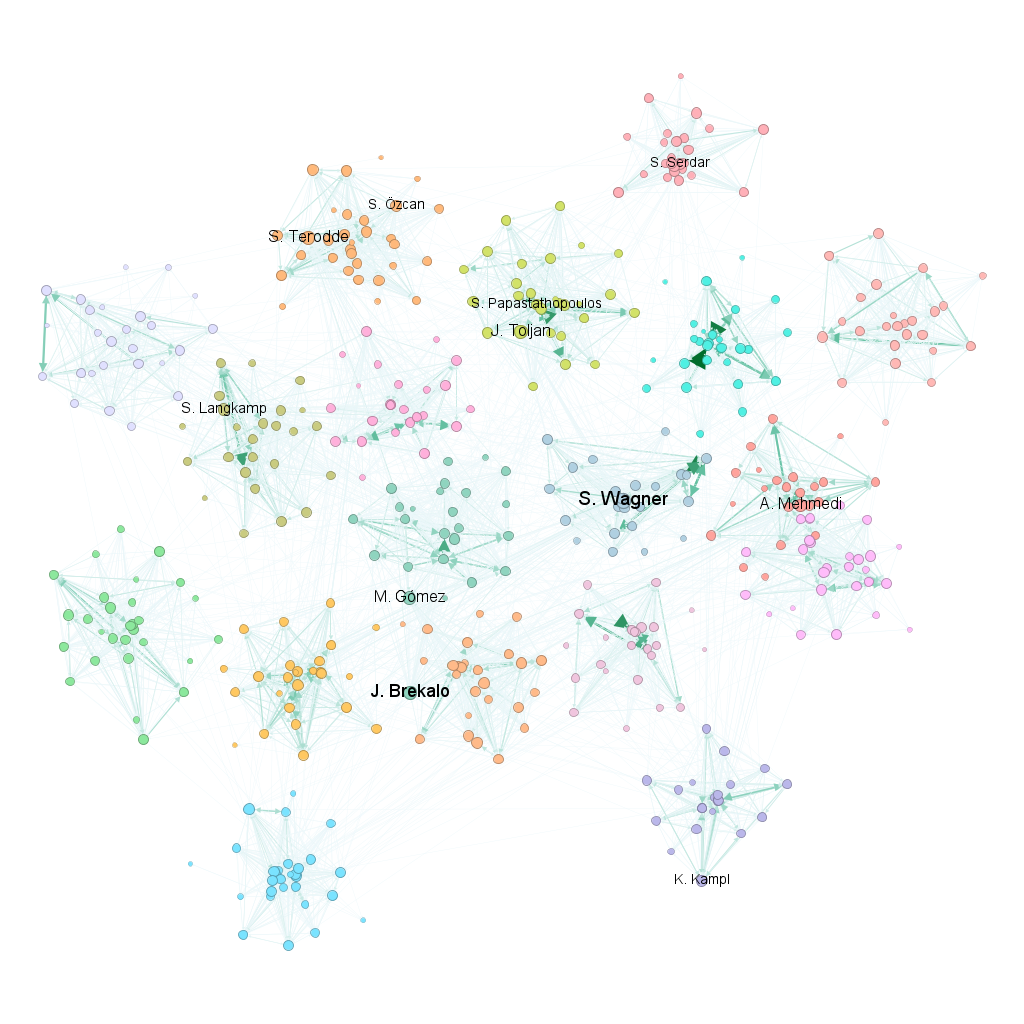
\includegraphics[width=0.9\linewidth,height=0.38\textheight,keepaspectratio]{figures/LE3/pass_network_full.png}
  \caption{Pass-Netzwerk (Beispiel). Knoten = Spieler, gerichtete Kanten = erfolgreiche Pässe, Breite typischerweise proportional zu \texttt{pass\_count}.}
  \label{fig:le3_pass_network_full}
\end{figure}

\begin{figure}[htbp]
  \centering
  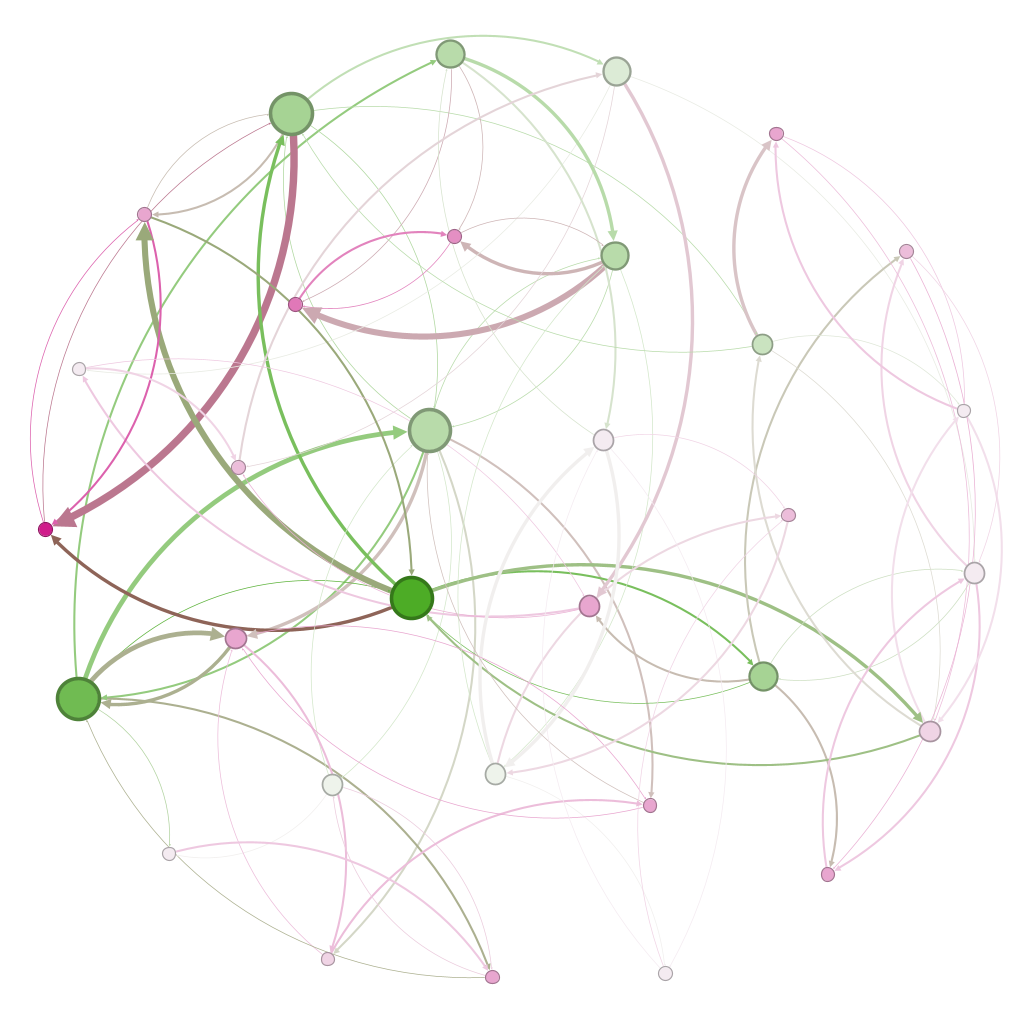
\includegraphics[width=0.9\linewidth,height=0.38\textheight,keepaspectratio]{figures/LE3/match_network_circular.png}
  \caption{Match-Netzwerk (Beispiel). Knoten = Teams, gerichtete Kanten = aggregierte Resultate zwischen Team-Paaren.}
  \label{fig:le3_match_circular}
\end{figure}

\begin{figure}[htbp]
  \centering
  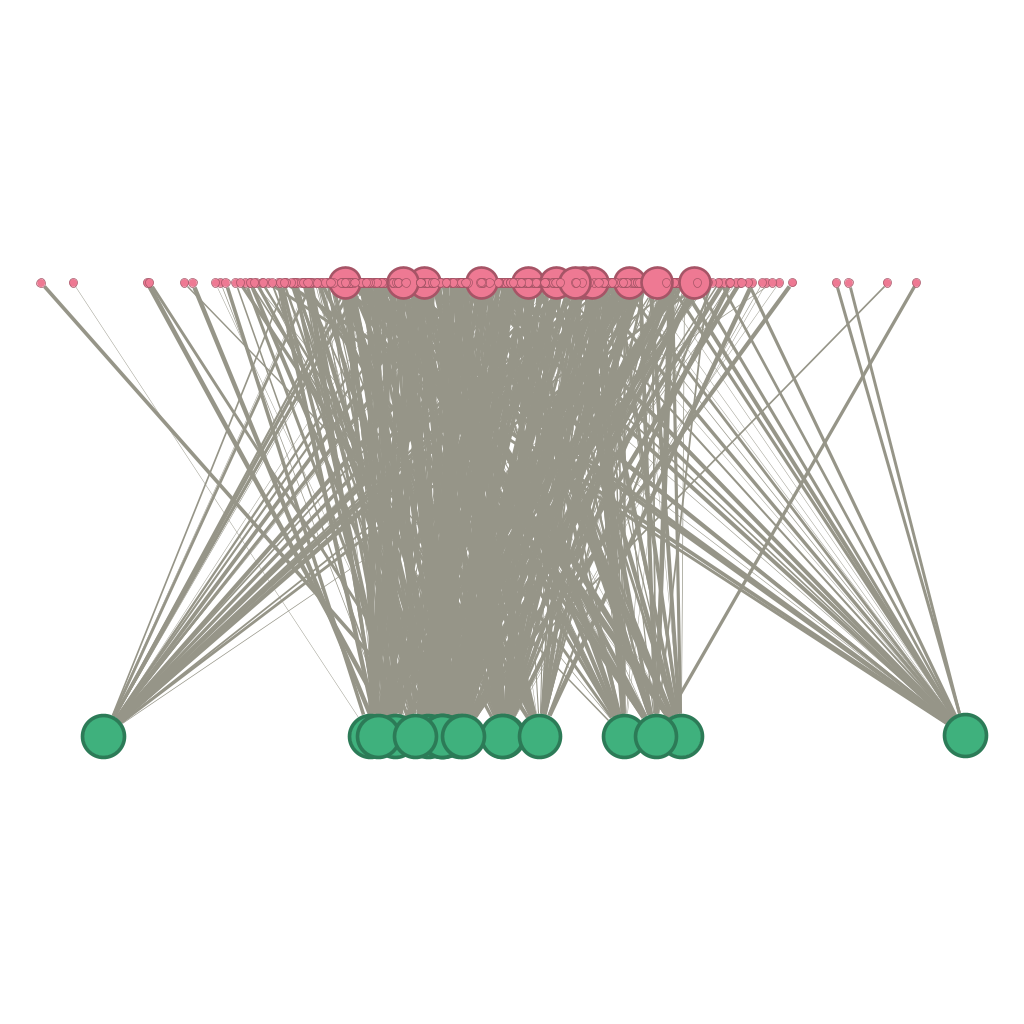
\includegraphics[width=0.9\linewidth,height=0.38\textheight,keepaspectratio]{figures/LE3/bipartite_network.png}
  \caption{Player--Team Two-Mode Netzwerk (vor Flattening). Spieler sind typischerweise genau einem Team zugeordnet (zwei bei Teamwechsel); Kantenbreite kodiert \texttt{matches\_together}.}
  \label{fig:le3_player_team_before}
\end{figure}

\begin{figure}[htbp]
  \centering
  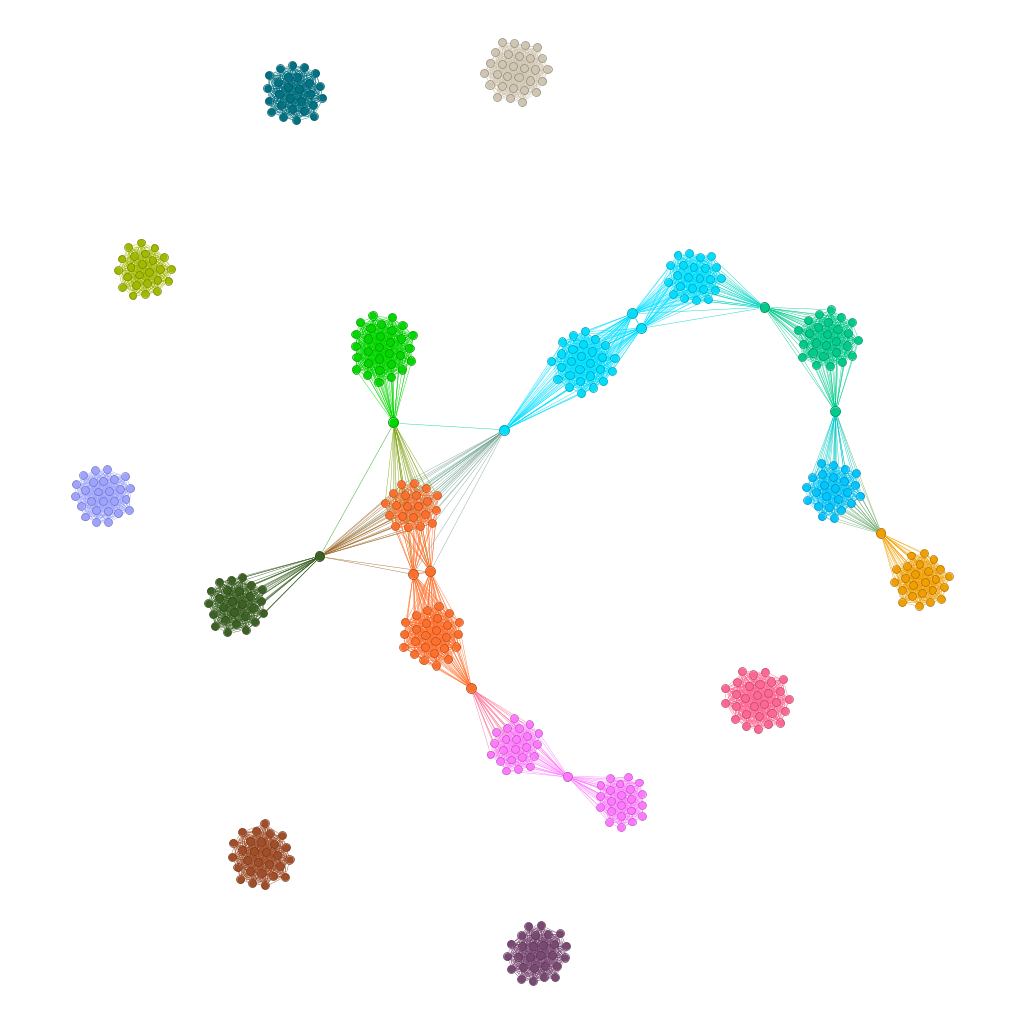
\includegraphics[width=0.9\linewidth,height=0.38\textheight,keepaspectratio]{figures/LE3/player_projection_network.png}
  \caption{Player--Player Netzwerk (nach Flattening / Projektion). Eine Kante entsteht durch gemeinsames Team; Gewichte akkumulieren gemeinsame Einsätze.}
  \label{fig:le3_player_team_after}
\end{figure}

\begin{figure}[htbp]
  \centering
  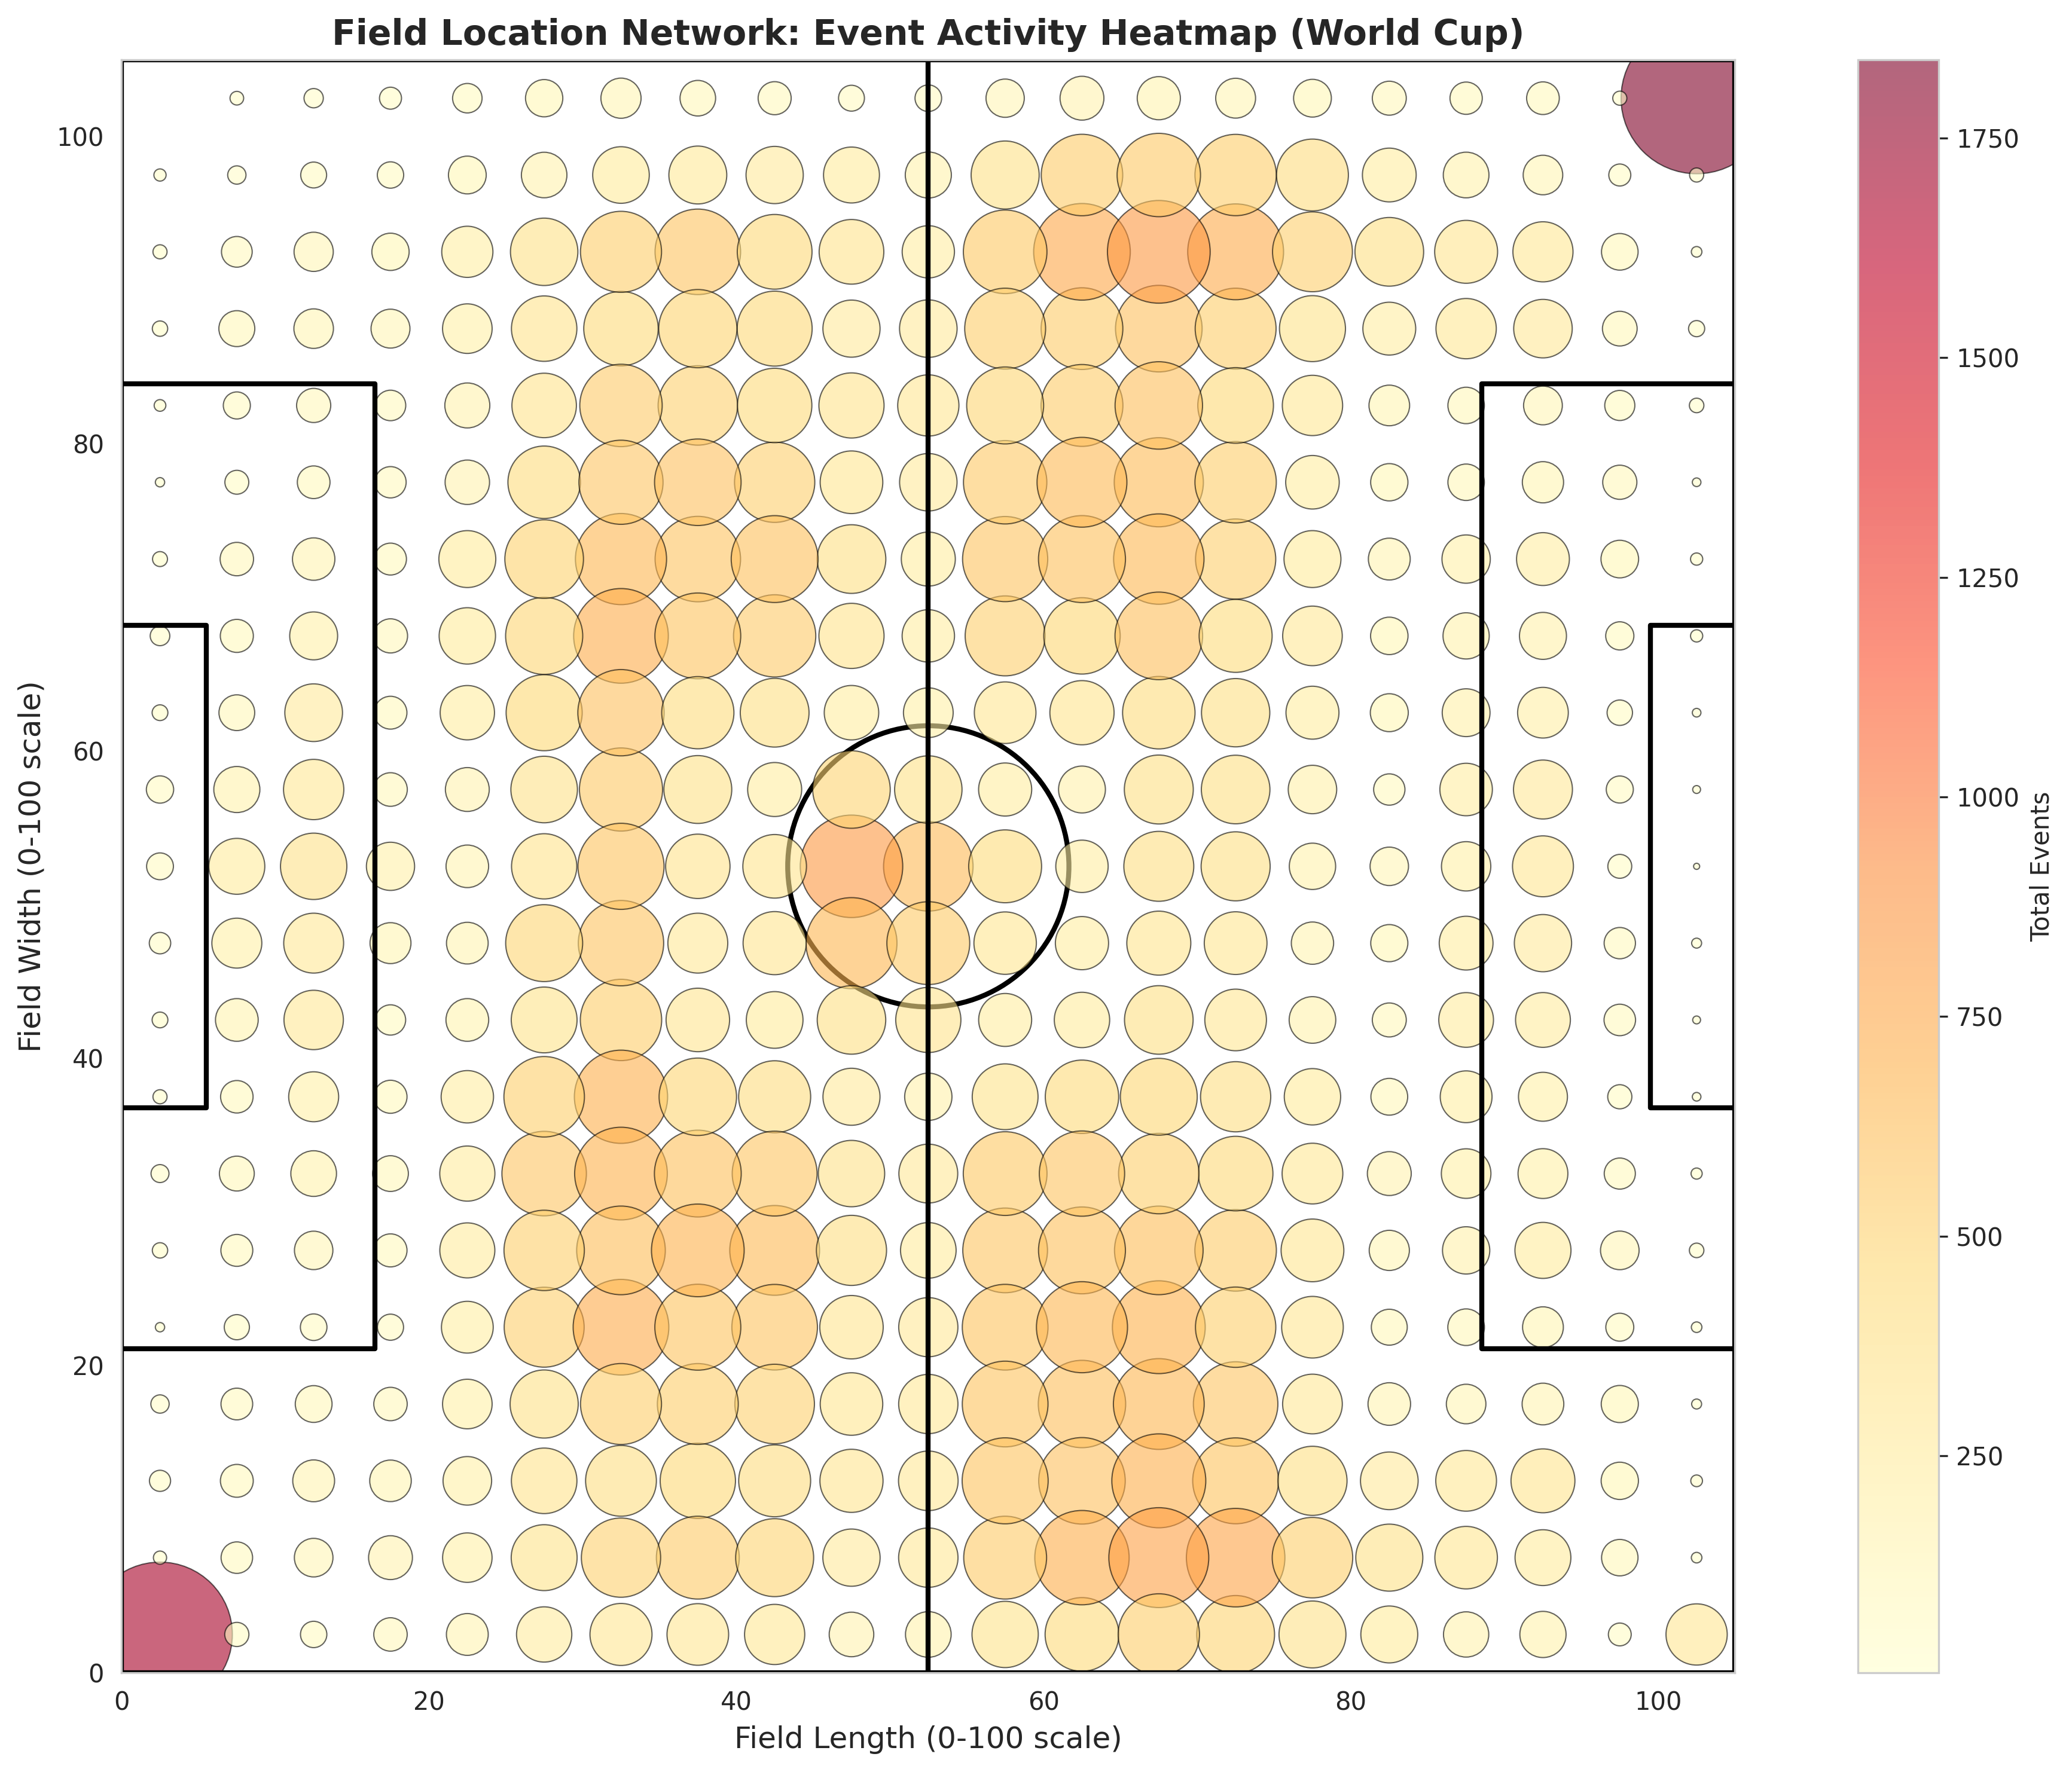
\includegraphics[width=0.9\linewidth,height=0.38\textheight,keepaspectratio]{figures/LE3/field_network_heatmap.png}
  \caption{Feld-Lokationsnetzwerk (Beispiel) als Heatmap. Farbe/Grösse kodieren Ereignisintensität in diskreten Feldzonen.}
  \label{fig:le3_field_heatmap}
\end{figure}

\subsection{Netzwerkfilterung}

In diesem Kapitel beschreiben wir, wie wir Filterung und Sichten (Local/Global/Ego) einsetzen, um aus grossen Netzwerken analysierbare Teilstrukturen zu extrahieren. Der Fokus liegt auf der praktischen Nutzung: welche Fragen lassen sich damit beantworten, und welche Visualisierungen stützen die Interpretation.

\subsubsection{Sichten: Local View, Global View, Ego-Netzwerk}

\paragraph{Local View (z.B. nur ein Team)}
Eine lokale Sicht extrahiert typischerweise ein Team-Subgraph aus dem Pass-Netzwerk (nur Pässe zwischen Spielern desselben Teams). Damit kann man z.B. untersuchen, ob die Stärke und Zentralisierung der teaminternen Verknüpfungen mit sportlichem Erfolg korrelieren (z.B. Punkte, Tore, Goal Difference).

\begin{figure}[htbp]
  \centering
  \includegraphics[width=0.9\linewidth,height=0.36\textheight,keepaspectratio]{figures/LE3/local_view_team_placeholder.png}
  \caption{\textbf{Platzhalter:} Local View eines Team-Subgraphs im Pass-Netzwerk (bitte passende Abbildung exportieren/benennen).}
  \label{fig:le3_local_view_team}
\end{figure}

\paragraph{Global View (z.B. Wettbewerb/League als Ganzes)}
Die globale Sicht betrachtet das komplette Netzwerk eines Wettbewerbs (z.B. gesamtes Match-Netz oder gesamtes Pass-Netz pro Competition). Sie dient dem Vergleich zwischen Competitions oder zur Einordnung von Extremwerten (z.B. Dichte, Komponenten, Gradverteilungen).

\begin{table}[h]
\centering
\caption{übersicht der konstruierten Netzwerke (Germany; aus \texttt{.gexf} berechnet)}
\label{tab:network_summary}
\begin{tabular}{lcccc}
	oprule
	extbf{Netzwerktyp} & \textbf{|V|} & \textbf{|E|} & \textbf{Dichte} & \textbf{Komponenten} \\
\midrule
Pass-Netzwerk & 473 & 8786 & 0.039354 & 8 \\
Match-Netzwerk & 18 & 306 & 1.000000 & 1 \\
Spieler-Team-Netzwerk & 492 & 503 & 0.004164 & 1 \\
Spieler-Projektion & 474 & 6803 & 0.060686 & 1 \\
\bottomrule
\end{tabular}
\end{table}

\begin{figure}[htbp]
  \centering
  \includegraphics[width=0.9\linewidth,height=0.36\textheight,keepaspectratio]{figures/LE3/global_view_placeholder.png}
  \caption{\textbf{Platzhalter:} Global View (z.B. Gesamtgraph eines Wettbewerbs, oder Vergleich mehrerer Competitions in einer Grafik).}
  \label{fig:le3_global_view}
\end{figure}

\paragraph{Ego-Netzwerk (Spielerfokus)}
Ego-Netzwerke isolieren die unmittelbare Umgebung eines Spielers (Ego) und sind hilfreich, um Rollen im Teamkontext zu interpretieren (z.B. als Connector/Hub) oder konkrete Passpartner-Strukturen zu visualisieren.

\begin{figure}[htbp]
  \centering
  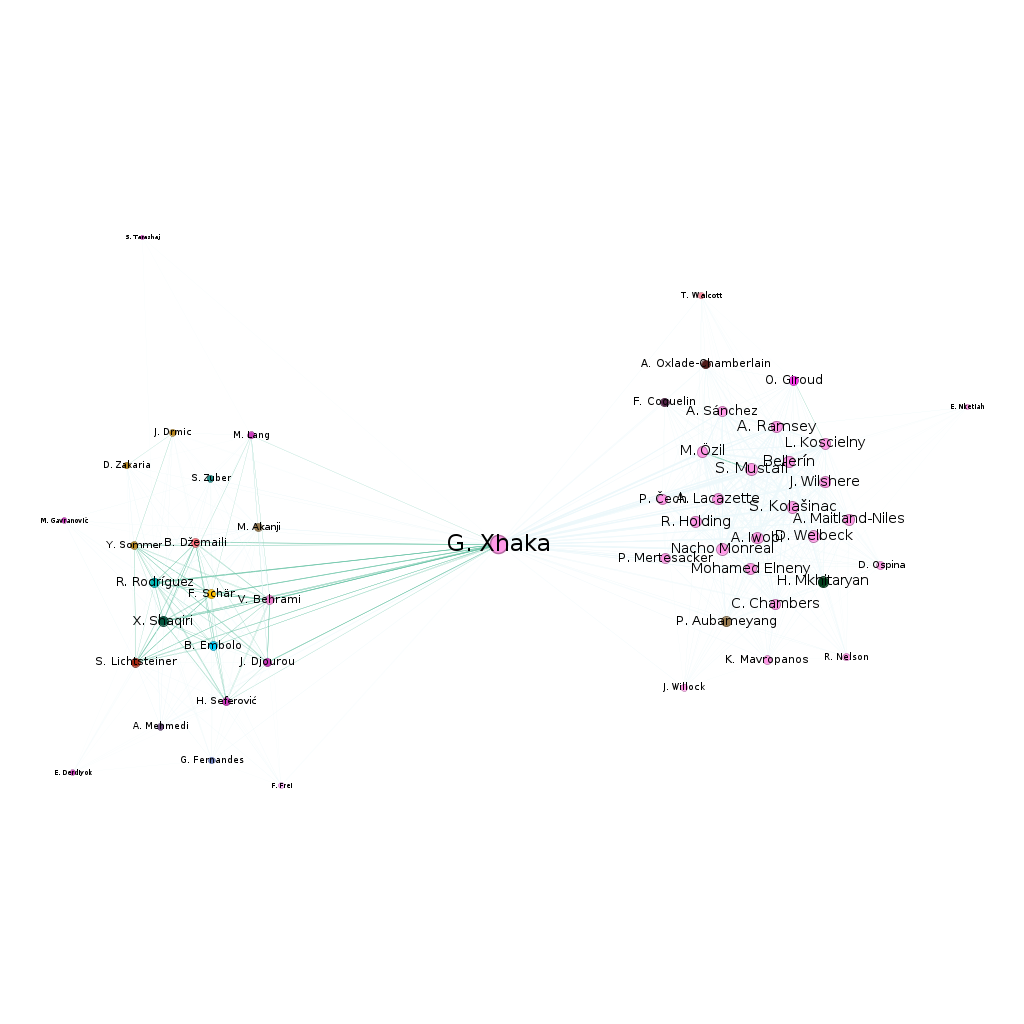
\includegraphics[width=0.9\linewidth,height=0.36\textheight,keepaspectratio]{figures/LE3/Ego_granitXhaka.png}
  \caption{Ego-Netzwerk von Granit Xhaka (\textbf{Platzhalter falls Datei noch fehlt:} bitte unter \texttt{figures/LE3/Ego\_granitXhaka.png} ablegen).}
  \label{fig:le3_ego_xhaka}
\end{figure}

\subsubsection{Filtern anhand von Kantenattributen}
Wir setzen Kantenattribut-Filter ein, um "Rauschen" zu reduzieren und stabilere Beziehungen hervorzuheben. Im Pass-Netzwerk ist das zentrale Filterkriterium typischerweise \texttt{pass\_count} (Mindestanzahl Pässe pro Kante); optional sind Filter nach Genauigkeit oder Distanz sinnvoll.

Für Germany zeigt die gewichtsbasierte Filterung (nach Entfernen isolierter Knoten) z.B.:
\begin{itemize}
  \item $w \geq 5$: 91.1\% Knoten, 71.9\% Kanten erhalten
  \item $w \geq 10$: 85.6\% Knoten, 56.2\% Kanten erhalten
  \item $w \geq 20$: 76.7\% Knoten, 36.8\% Kanten erhalten
\end{itemize}

\begin{figure}[htbp]
  \centering
  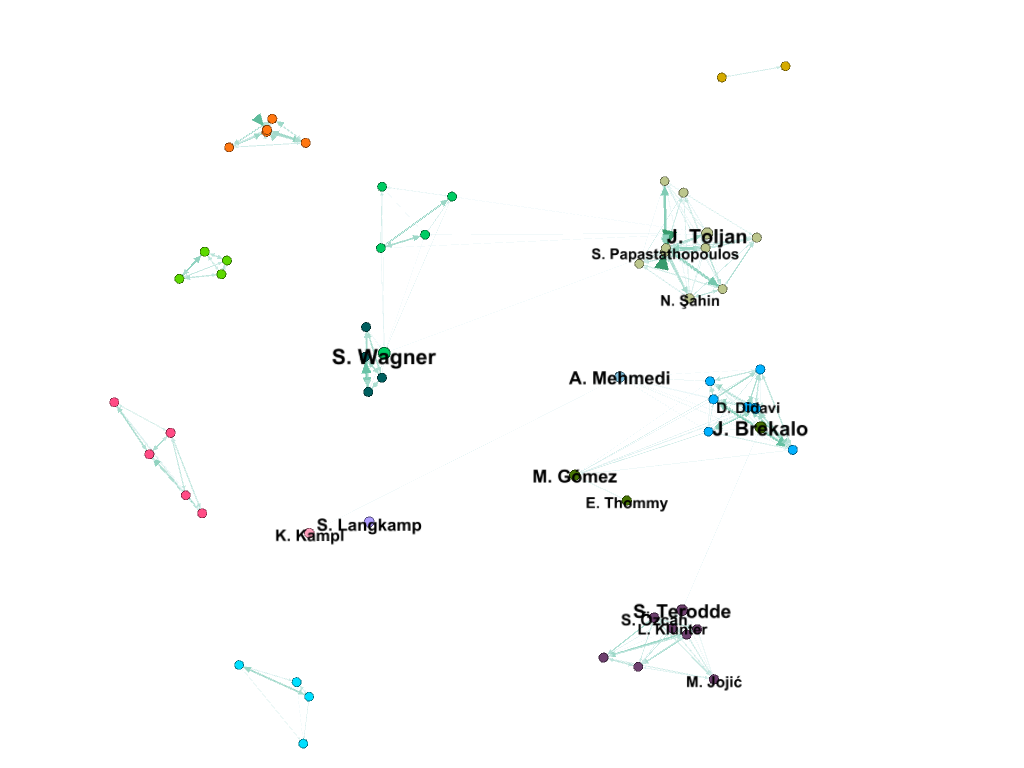
\includegraphics[width=0.9\linewidth,height=0.36\textheight,keepaspectratio]{figures/LE3/pass_network_filtered.png}
  \caption{Filterung nach Kantenattribut (Beispiel). \textbf{Falls diese Abbildung nicht die Filterkurve zeigt:} bitte eine passende Visualisierung exportieren und den Dateinamen hier anpassen.}
  \label{fig:le3_edge_attr_filter}
\end{figure}

\subsubsection{Offene Visualisierungen (benötigte Exporte)}
Wenn du willst, kann ich die Platzhalter direkt auf konkrete Dateinamen/Abbildungsunterschriften anpassen. Aktuell fehlen im Repo nur die Grafiken für:
\begin{itemize}
  \item Local View eines konkreten Teams (Pass-Subgraph)
  \item Global View (z.B. Competition-Vergleich oder Gesamtgraph als Plot)
\end{itemize}
Sag mir einfach, welche Competition/Teams du zeigen möchtest (und ob du eher Gephi-Viz oder Matplotlib/Seaborn-Plots bevorzugst).
  \centering
